\documentclass{vilniustech}
\vilniustechsetup{
    university={Vilniaus Gedimino technikos universitetas},
    faculty={Fundamentinių mokslų fakultetas},
    cathedral={Informacinių Sistemų katedra},
    workTitle={Kompiuterių tinklų ir operacinių sistemų sauga},
    workType={Įvadinė užduotis},
    workAuthorName={Aurimas Šakalys},
    workAuthorGroup={ITSfm-22},
    workRecipient={lektorius Vitalijus Gurčinas}
}
\addbibresource{bibliography.bib}
\VTDocumentBegin


\section{Bendra tinklo topologija}

Įvadinė kurso užduotis buvo įgyvendinta naudojant GNS3 įrankį. Užduoties uždaviniai skamba taip:

\begin{itemize}
\item Sukurti virtualią tinklo topologiją, kurioje būtų:
\begin{itemize}
    \item{Du maršrutizatoriai}
    \item{Du komutatoriai}
    \item{Du tinklo segmentai}
    \item{Šeši įrenginiai, kurių vienas - bevielis}
\end{itemize}
\item Sujungti ir sukonfiguruoti šiuos virtualius įrenginius
\end{itemize}

Čia, dėl trūkumų bevielių įrenginių simuliacijai GNS3 įrankyje, pasirinkau viename tinklo segmente pridėti papildomą komutatorių, kuris atstotų bevielį prieigos tašką.

Įgyvendintą topologiją galima pamatyti \ref{fig:topology} paveikslėlyje. Čia tariame, jog yra reikmė sujungti dviejų biurų vidinius tinklus. Vienas iš šių biurų yra didesnis, turintis didesnį kiekį kambarių, kas reikalauja ir didesnio kiekio komutatorių. Kitas yra vieno kambario biuras.

\begin{figure}[H]
\begin{center}
    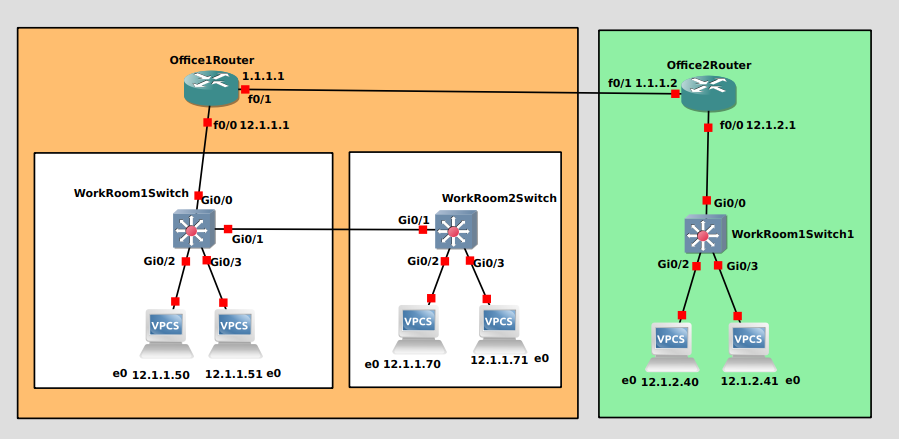
\includegraphics[height=8cm]{img/topology.png}
    \caption{Bendra tinklo topologija}
    \label{fig:topology}
\end{center}
\end{figure}

\section{GNS3 virtualaus tinklo įrenginiai}

Tinkle yra nauojami trijų tipų įrenginiai:

\begin{itemize}
    \item VPCs 
    \begin{itemize} 
        \item Gerokai supaprastintas asmeninio kompiuetrio modelis, kuris geba atlikti bazines tinklo užduotis (\ref{fig:vpcs} pav.) ir sukonfiguruoti savo tinklo sąsają. Tiek funkcionalumo užtenka, norint patikrinti, ar iš vieno tinklo mazgo galime pasiekti kitus.
    \end{itemize}
    \item Cisco IOS Layer-2 komutatorius
    \begin{itemize} 
        \item Virtualus Cisco komutatorius, gebantis atlikti pagrindinius komutatoriaus uždavinius - t.y. tinkamai nukreipti gaunamus paketus lokaliame tinkle. Šis komutatorius taip pat turi ir Layer 3 funkcionalumus, tačiau šiame įgyvendinime šis funkcionalumas yra deleguotas maršrutizatoriams.
    \end{itemize}
    \item Cisco 3725 maršrutizatorius
    \begin{itemize} 
        \item Virtualizuotas, fizinis maršutizatorius.
    \end{itemize}
\end{itemize}

\begin{figure}[H]
\begin{center}
    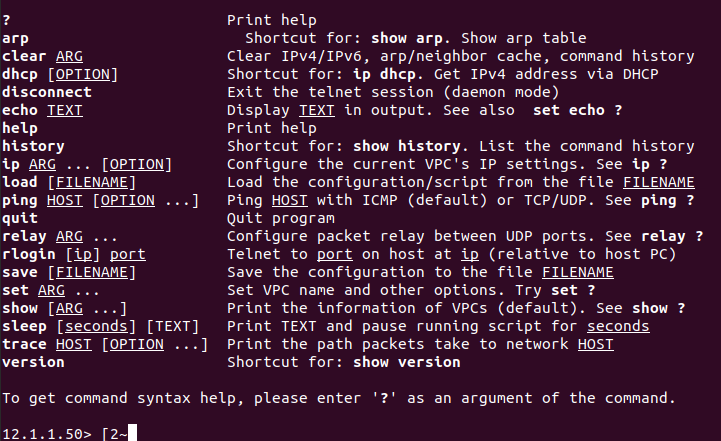
\includegraphics[height=8cm]{img/vpcs.png}
    \caption{Komandas kurias palaiko VPC}
    \label{fig:vpcs}
\end{center}
\end{figure}

\section{Tinklų konfiguracija}

Tariame, kad šie konfiguruojami tinklai neturi būti prijungti prie interneto. Dėl šios priežasties, mūsų darbas gerokai palengvėja, kadangi mums nebereikia NAT funkcionalumo ir kiekvienam įrenginiui tinkle galime suteikti unikalų IP adresą.

Oranžiniam ofisui yra skirtas 12.1.1.0/24 tinklas, čia yra sukonfiguruoti keturi galiniai mazgai. \textit{Default gateway} gauna pirmajį tinklo adresą - 12.1.1.1.

Žaliam ofisui yra skirtas 12.1.2.0/24 tinklas, čia yra sukonfiguruoti du galiniai mazgai. \textit{Default gateway} taip pat gauna pirmajį tinklo adresą - 12.1.2.1.

Kadangi maršrutizatoriai nėra prijungti į internetą (ar kitą, didelį WAN tinklą), visa maršutizatorių konfiguracija yra statinė. Pirmasis maršutizatorius paketus skirtus 12.1.1.0/24 siunčia į šį tinklą (kadangi jis tiesiogiai su juo sujungtas), o paketus skirtus 12.1.2.0/24 siunčia į antrajį maršutizatorių IP adresu 1.1.1.2. Antrasis maršrutizatorius atvirkščiai - paketus skirtus 12.1.2.0/24 siunčia į šį tinklą, o paketus skirtus 12.1.1.0/24 siunčia pirmąjąm maršutizatoriui IP adresu 1.1.1.1. Maršrutizatorių maršrutų konfiguraciją galima pamatyti \ref{fig:router} paveikslėlyje.

\begin{figure}[H]
\begin{center}
    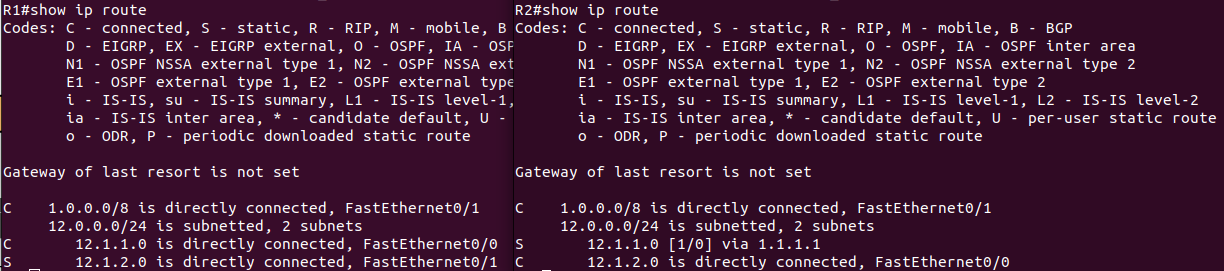
\includegraphics[width=16cm]{img/router.png}
    \caption{Maršrutų konfiguracija}
    \label{fig:router}
\end{center}
\end{figure}

\section{Tinklo testavimas}

Norint įsitikinti, jog mūsų atlikta konfiguracija yra veikianti, atliksime du testus:

\begin{itemize} 
    \item iš 12.1.1.50 mazgo bandysime pasiekti 12.1.2.40 mazgą
    \item iš 12.1.2.41 mazgo bandysime pasiekti 12.1.1.70 mazgą
\end{itemize}

\begin{figure}[H]
\begin{center}
    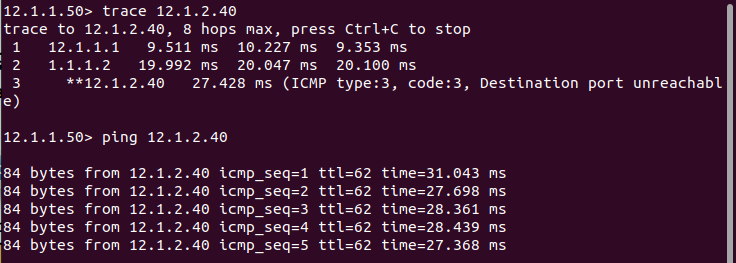
\includegraphics[width=16cm]{img/test1_ping.png}
    \caption{Pirmojo testo \textit{trace} ir \textit{ping} komandų rezultatas}
    \label{fig:t1ping}
\end{center}
\end{figure}

\begin{figure}[H]
\begin{center}
    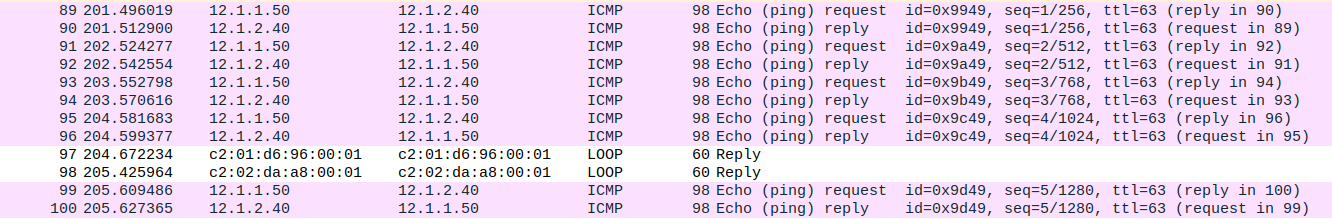
\includegraphics[width=16cm]{img/test1_wireshark.png}
    \caption{Pirmojo testo tinklo paketai}
    \label{fig:t1wireshark}
\end{center}
\end{figure}

Kaip galime matyti \ref{fig:t1ping} paveikslėlyje, kadangi siunčiami paketai nėra lokaliam tinklui (12.1.1.0/24), šis paketas yra siunčiamas \textit{default gateway}, IP adresu 12.1.1.1. Šis, pagal savo konfiguraciją mato, jog paketas skirtas 12.1.2.0/24 tinklui, todėl paketą išsiunčia antrąjąm maršrutizatoriui adresu 1.1.1.2. Čia patekęs paketas yra siunčiamas į 12.1.2.0/24, kur pasiekia galutinį mazgą. Šiuos paketus taip pat galime matyti \ref{fig:t1wireshark} paveikslėlyje.

\begin{figure}[H]
\begin{center}
    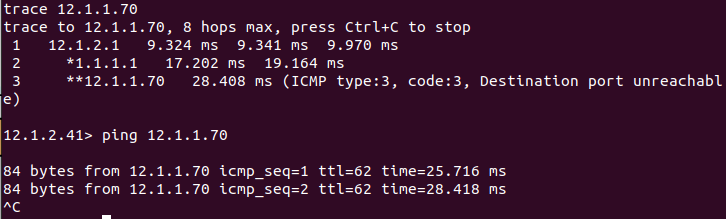
\includegraphics[width=16cm]{img/test2_ping.png}
    \caption{Antrojo testo \textit{trace} ir \textit{ping} komandų rezultatas}
    \label{fig:t2ping}
\end{center}
\end{figure}

\begin{figure}[H]
\begin{center}
    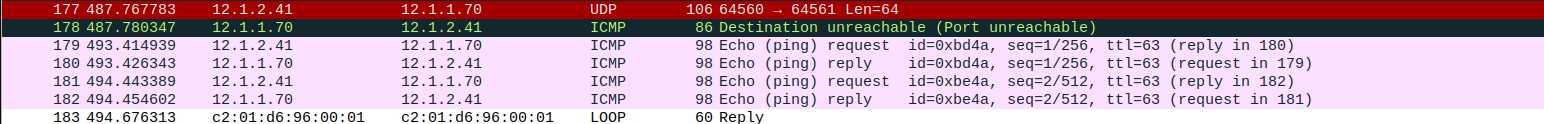
\includegraphics[width=16cm]{img/test2_wireshark.png}
    \caption{Antrojo testo tinklo paketai}
    \label{fig:t2wireshark}
\end{center}
\end{figure}

Kaip galime matyti \ref{fig:t2ping} paveikslėlyje, kadangi siunčiami paketai nėra lokaliam tinklui (12.1.2.0/24), šis paketas yra siunčiamas \textit{default gateway}, IP adresu 12.1.2.1. Šis, pagal savo konfiguraciją mato, jog paketas skirtas 12.1.1.0/24 tinklui, todėl paketą išsiunčia pirmąjam maršrutizatoriui adresu 1.1.1.1. Čia patekęs paketas yra siunčiamas į 12.1.1.0/24, kur pasiekia galutinį mazgą. Šiuos paketus taip pat galime matyti \ref{fig:t2wireshark} paveikslėlyje.

Iš šių rezultatų galime spresti, jog kiekvienas tinklo mazgas gali pasiekti kitus tinklo mazgus, net ir kituose tinklo segmentuose.
\VTDocumentEnd